\section{Experiment}
\label{experiment}
\subsection{Setup}
Our experimental data consists of running small programs under 4 different configurations: with contracts and the JIT, with no contracts and the JIT, with contracts and no JIT, and finally with no contracts and no JIT.
We disabled the JIT using the Racket command-line flag \mono{--no-jit} and disabled contracts by editing the \mono{racket/contract} source code\textemdash wherever contracts were applied, we replaced the actual contract with a trivial \mono{any/c} contract.\footnote{See \sect{disabling-contracts} for a more on our strategy for disabling contracts.}

The seven programs we collected data for are taken from Project Euler~\cite{project-euler} and the artifact by Nyugen et~al. on soft contracts~\cite{soft-contracts}.
We wrote the four Project Euler (PE) solutions ourselves and later added contracts to protect individual functions exactly how type signatures would guard the functions in a statically-typed language.\footnote{We chose these 4 problems arbitrarily.}
The three games we took from the soft contracts repository~\cite{soft-contracts-repo} were implemented as a collection of modules.
Contracts only protect module boundaries, not functions within a module.
Incidentally, this style of using contracts on modules rather than functions is the preferred Racket way; see \sect{types-of-boundaries}.

We ran each of these 8 benchmark programs on a modern desktop using Racket version 6.1.1.5 and collected the CPU time taken for the run.\footnote{CPU time was obtained by calling Racket's built-in \mono{time} function.}
To address potential outliers, we ran each benchmark 30 times on each configuration of Contracts and JIT.
Note that we started a new Racket VM for each of the 30 runs; our experiment does not measure differences between startup and steady-state performance.

\subsection{Results}
Figures~\ref{runtimes} and~\ref{speedups} document our results.
We discuss these figures in turn.

\begin{figure}[t]
  \begin{center}
  \hspace*{-1.5cm}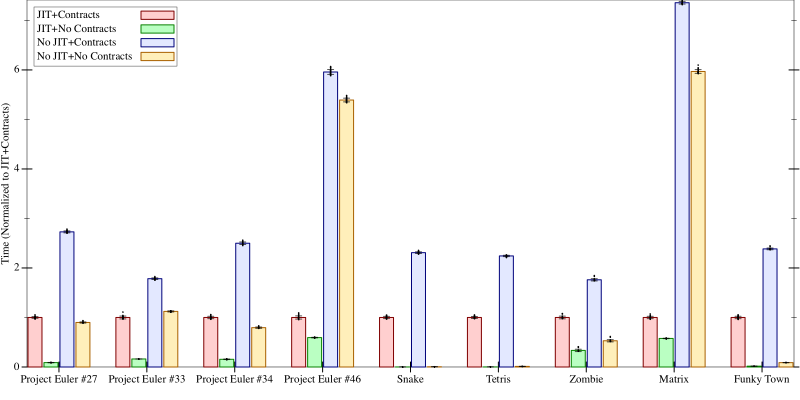
\includegraphics[width=15cm]{data/normalized-runtimes.png}
  \caption{All experiment runtimes, normalized to contracts + JIT runtime.}
  \label{fig:runtimes}
  \end{center}
\end{figure}

\fig{runtimes} shows the aggregate runtime for each experiment on each of the 4 configurations, normalized to the ``Contracts + JIT'' running time.
The bars additionally include their 95\% confidence interval.
The confidence intervals suggest minimal variation among the 30 trials we collected data for.
This suggests that our benchmarks are ``well-behaved'' in the sense that both contract overhead and JIT optimizations apply uniformly across trials, and that we are justified in extrapolating our data to more general settings.

From this chart, we conclude that contracts are responsible for at least an order of magnitude slowdown under normal execution.
With the JIT disabled, the runnning-time effects of contracts are generally less severe but still significant.
We also conclude that the JIT is responsible for large speedups regardless of whether contracts are on or off.
Regarding the individual projects, we first note that our solution to Project Euler \#46 benefits tremendously from the JIT.\footnote{Indeed, the appendix notes that this benchmark does a lot of redundant computation\textemdash it computes the first 10,000 primes using the Sieve of Eratosthenes.}
Snake and Tetris, from the soft contracts repo, finish very quickly with contracts disabled.
This suggests that these benchmarks were divided into contracted modules too agressively, and may not be indicative of the contract overhead one might see naturally.

\newpage
\begin{figure}[!thb]
  \begin{center}
  \vspace*{-2cm}\hspace*{-1cm}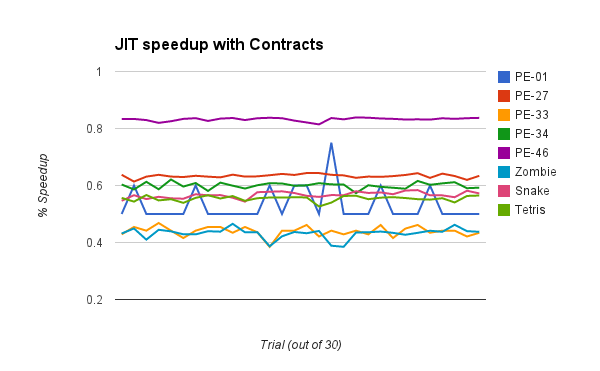
\includegraphics[width=\textwidth]{data/contracts-jit-speedup.png}

  \vspace*{1cm}\hspace*{-1cm}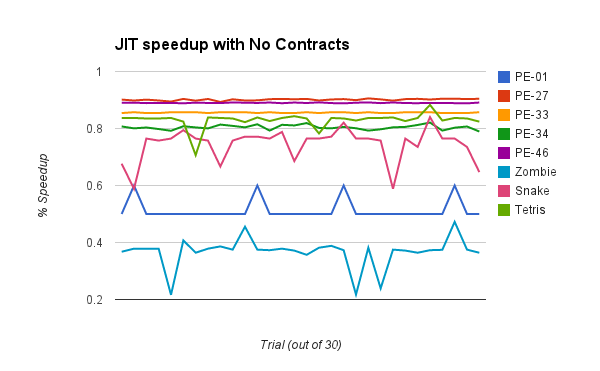
\includegraphics[width=\textwidth]{data/nocontracts-jit-speedup.png}
  \caption{Percent difference in runtimes with and without the JIT}
  \label{speedups}
  \end{center}
\end{figure}

\fig{speedups} shows the percent difference in runtimes without the JIT versus those with the JIT.
The two charts displayed vertically in this figure measure the increases with / without contracts, respectively.
Each chart gives the precise data for each of the 30 trials.

Besides \#46, all the Project Euler questions see a large, consistent speedup after removing contracts.
Thus we conclude that the contracts did hinder the JIT's ability to optimize (despite offering more ``redundant computation'' to potentially reduce).
The anomaly, Problem 46, is consistently optimized.
This makes sense considering the amount of redundant computation it contains.

The soft contracts benchmarks are a little more interesting.
Tetris is similar to our Project Euler benchmarks in that it clearly optimizes better without contracts.
On the other hand Zombie, the benchmark using the most higher-order contracts, is optimized relatively poorly regardless of whether contracts are erased.
In the case of no contracts these optimizations take effect more unpredictably.
These results suggest that an object-oriented style of programming is less amenable to Racket's optimizations.
Finally, Snake has the strangest results.
On average, the JIT optimizes more with contracts removed; however, the magnitudes of these optimizations are more variable.
We do not have a good explanation for this result.
Intuitively, Snake should behave like Tetris as both use a random number generator for small game components (spawning new items / pieces) and are coded as traditional functional programs.

To summarize, our results suggest that the JIT optimizes better with contracts removed.
This is modestly surprising because we expect the JIT to optimize repeated contract-checks, however the changes contracts cause to a program's execution pattern apparently bear a more significant cost.

